
\section{Data Preparation}
Kaggle is a public platform which provides various types of data for research purpose. The dataset 'foodRecSys-V1' used in this thesis is received from Kaggle \cite{48}. This dataset consists of three files. The 'core-data\_recipe.csv' file has all information about recipes such as 'recipe\_id', 'recipe\_name', 'image\_url', 'ingredients', 'cooking\_directions', 'nutritions' as shown in \autoref{fig:raw_recipes_head}. It has $45630$ recipes with $6$ columns as per \autoref{fig:raw_recipes_shape}.

\begin{figure}[H]
	\centering
	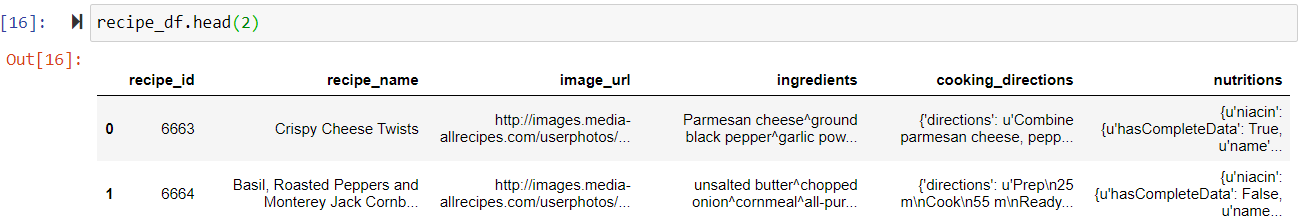
\includegraphics[width=0.8\linewidth]{raw_recipes_head}
	\caption{Raw Recipe Data}
	\label{fig:raw_recipes_head}
\end{figure}

\begin{figure}[H]
	\centering
	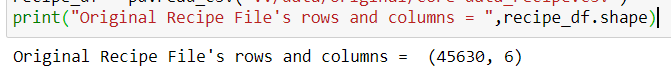
\includegraphics[width=0.8\linewidth]{raw_recipes_shape}
	\caption{Rows and Columns of original recipe's file}
	\label{fig:raw_recipes_shape}
\end{figure}

\noindent The other two files 'core-data-train\_rating.csv' and 'core-data-test\_rating.csv' provide user interactions with recipes. User interaction refers to a record in the file such as a user has given a rating to a recipe as depicted in \autoref{fig:raw_ratings_head}. These two files are combined and formed a single file that has all user interactions.  It has $960386$ users-recipes interactions and $4$ columns, 'user\_id', 'recipe\_id', 'rating', 'dateLastModified' as shown in
 \autoref{fig:original_interactions_shape}.

\begin{figure}[H]
	\centering
	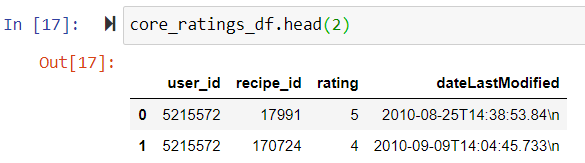
\includegraphics[width=0.8\linewidth]{raw_ratings_head}
	\caption{Raw User-Interaction Data}
	\label{fig:raw_ratings_head}
\end{figure}

\begin{figure}[H]
	\centering
	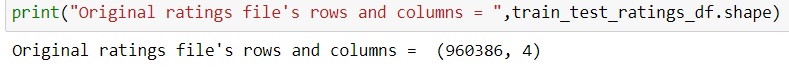
\includegraphics[width=0.8\linewidth]{original_interactions_shape}
	\caption{Rows and Columns of original user-recipes interactions }
	\label{fig:original_interactions_shape}
\end{figure}  


\subsection{Features Extraction}
A content-based filtering algorithm relies on the contents of the items. In our dataset, recipes are items that are rated by users. To recommend any recipe for a user, it is important to understand the features of the recipe that are relevant for a user. This thesis considers 'Ingredients', 'Cooking Method', 'Calories' and 'Diet Labels' features to find similarities between recipes.

\subsubsection{Ingredients Extraction}
The recipe's data received from Kaggle has the ingredients column in a clean format at a certain level. To get a single ingredient for each recipe, the "NLTK" library has been used. It tokenizes sentences into words. Raw ingredients data has many words that are irrelevant in predicting similarity between ingredients such as 'white' from 'white eggs', 'frozen', 'thawed', 'piece'. Such custom keywords are added in a recipe\_stopwords list and removed them from ingredients to make ingredients very specific. The difference between raw ingredients and cleaned ingredients is illustrated in \autoref{fig:raw_ingredients} \autoref{fig:clean_ingredients}. Irrelevant words such as 'thawed' and 'white' present in the first column of the pre-processed ingredients column have been removed in post-processed ingredients.

\begin{figure}[H]
	\centering
	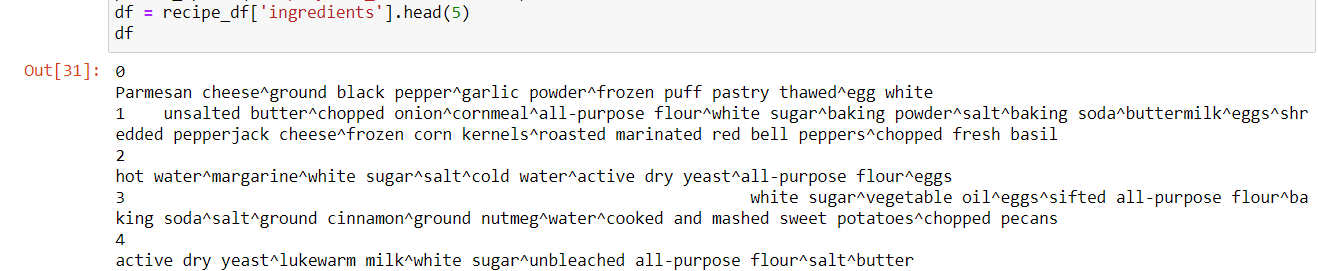
\includegraphics[width=0.9\linewidth]{raw_ingredients}
	\caption{Pre-Processed Ingredients }
	\label{fig:raw_ingredients}
\end{figure}  


\begin{figure}[H]
	\centering
	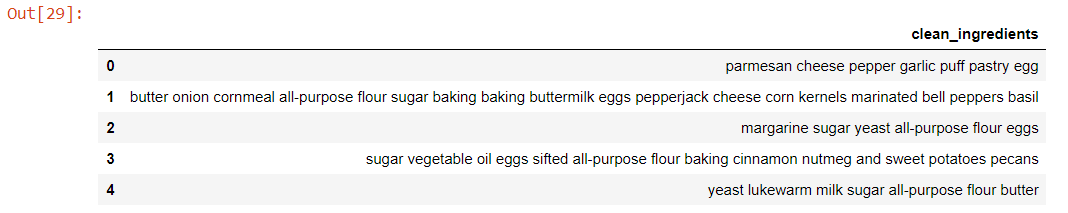
\includegraphics[width=0.9\linewidth]{clean_ingredients}
	\caption{Post-Processed Ingredients }
	\label{fig:clean_ingredients}
\end{figure}  

\subsubsection{Cooking Method Extraction}
\subsubsection{Calories Extraction}
\subsubsection{Diet Labels Extraction}